\section{Packet}
Grundstäzlich ist ein Packet ein Zusammenschluss von mehreren Quests. Dadurch soll es Erstellern von Quests erlaubt sein, die Aufgaben in Bereiche zu gliedern. Programmtechnisch wird das so gehandhabt, dass mehrere Quest, welche in einem Ordner zusammengefasst werden, ein Package bilden.

\subsection{Organisation von Packages und Quests}
\begin{figure}[h] 
  \centering
     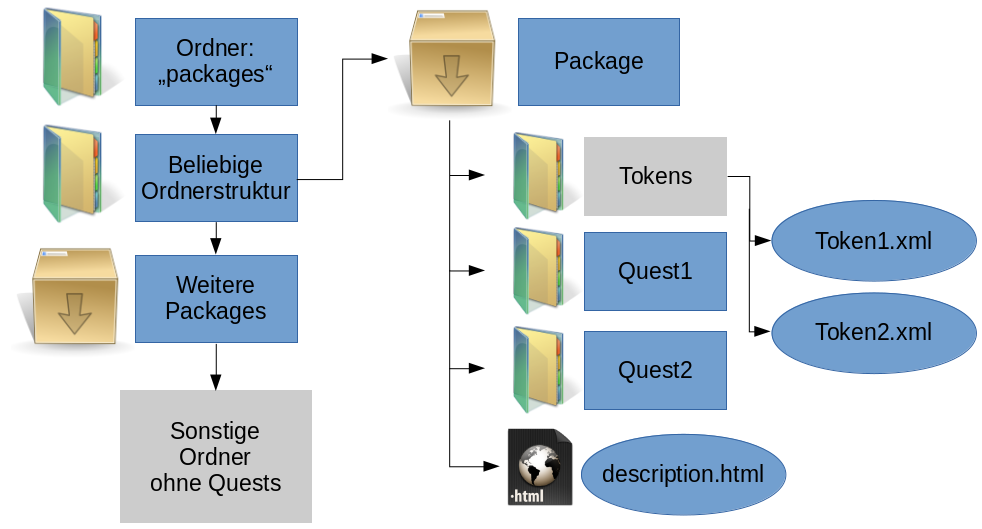
\includegraphics[width=0.8\textwidth]{./media/images/quest/ordnerstruktur.png}
  \caption{Beispielhafte Darstellung einer Ordnerstruktur}
  \label{fig:package_ordnerstruktur_1}
\end{figure}
Wie aus dem Bild zu erkennen sein sollte, können Packages beliebig Organisiert sein. Sobald ein Ordner auftritt welcher keine Quest beinhaltet wird dieser von der Auswahl ausgeschlossen. 
Ein Package beinhaltet somit mehrere Quests.

Eine beliebige Ordnerstruktur kann auch mehrere Packages beinhalten. Hierbei können auch übergeordnete Packages erstellt werden. Dies hat vorallem den Sinn dadurch, wenn man Packete wiederum in mehrere Kapitel unterteilen will.

Ein Ordner, in der Package-Auswahl, kann auch wie eine Quest eine Beschreibung “description.html”, und ein “style.css” beinhalten.

Im Programm, werden die Packages und Quests automatisch anhand des Ordnernamens aufsteigend sortiert. Somit ist es für Ersteller von Packages einfach, diese in die gewünschte Reihenfolge zu bringen.